

The following results come  from a standard Python 2.7 interpreter
(not PyPy) running on a 2.6 GHz Mac Os/X with 4 GB of ram.
For NSGA-II,
we used the out-of-the-box version from DEAP, https://github.com/DEAP/deap.


In the following, we compared WICKED's results with
that of NSGA-II~\cite{deb00}.  NSGA-II is a genetic
algorithm (GA) with a highly optimized {\em select}
operator: \bi
\item Each generation builds generation $G+1$ by {\em selecting} better
individuals, {\em combining} some of their parts, then 
{\em mutating} the results 
(a little).
\item NSGA-II is a GA whose {\em select} operator 
uses a non-dominating sort
procedure to divide the solutions into {\em bands}
where {\em band}$_i$ dominates all of the solutions
in {\em band}$_{j>i}$ (and NSGA-II favors the
least-crowded solutions in the better bands).
\ei
One reason to favor NSGA-II as our comparison optimizer is 
 {\em repeatability}. 
Many multi-objective optimizers as MOEA/D~\cite{zhang07} 
and PSO~\cite{Poli07particleswarm}
are really {\em frameworks} within 
which an engineer has free reign to make numerous decisions
(evidence: review papers list dozens of variants on  PSO and MOEA/D ~\cite{V.Sedenka2010,5601760}).
Hence, in terms of {\em repeatability}, it can better to use precisely defined algorithms like NSGA-II.

Other reasons to use NSGA-II are that (a)~it is very widely used 
and (b)~there is no clear
consensus that some other algorithm is better.
When selecting a comparison algorithm,
we reached out to our SBSE colleagues to
find
which algorithms are accepted as ``best''.  However, no consensus was found.
On the other hand, it can be shown that NSGA-II is widely used.
In 2013, Sayyad and Ammar~\cite{sayyad13c} surveyed 36 SBSE papers where $\frac{21}{36}$
used NSGA-II  (of the others, 4 used some home-brew genetic algorithm and the remainder
each used some MOEA not used by any other paper).


\subsection{Runtimes}

Standard MOEAs require at least $N^2$ comparisons
between $N$ candidates, for each generation $G$ of the evolution. In theory,
WICKED is much faster than that:
\bi
\item The current implementation of WICKED uses $G=1$
since its recommendations are the results of one analysis of the data
(in future work, we plan to explore an iterative evolutionary version of the 
algorithm).
\item All the sub-routines of WICKED take near linear-time (the
slowest is CART that must sort all examples at each level of its trees).
\ei
On experimentation, WICKED's runtimes are consistent with its
theoretical properties. \fig{pomtimes} show the effect on runtimes
of increasing the initial population size for WICKED and NSGA-II.
The solid lines denote WICKED's performance: note that they are always less
that those seen with NSGA-II. 
The effect that WICKED runs faster than standard optimizers, is most
pronounced in the more complex models. In the POM3 results, some of the POM3 variants
take 100s of seconds to terminate. The same problems are handled by WICKER in
under one minute. 


% XXXnaveen
% for the runtime figures
% change CT to WICKED
% add space after label some xomo gr not xomogr
% delete all and delete os (so only 3 lines per optimizer)
% 2) any explnation for the spike in nsga at P=400?
% 3) are these repeats over 20 runs?
% 4) please confirm. popSize=200?

\begin{figure}
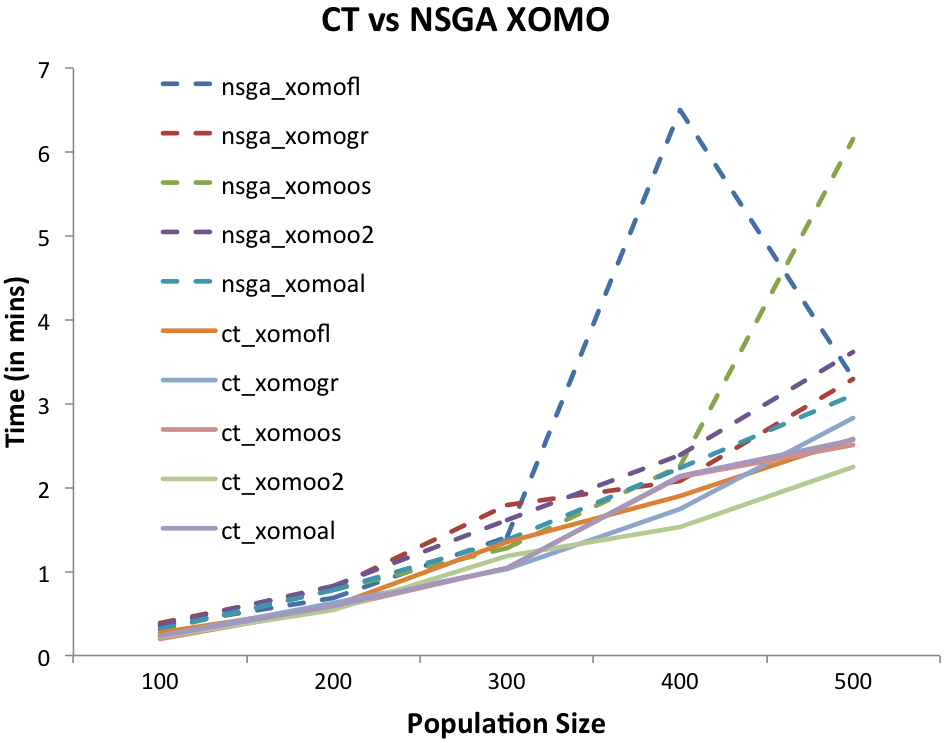
\includegraphics[width=6cm]{naveen/figures/xomotimes.png}
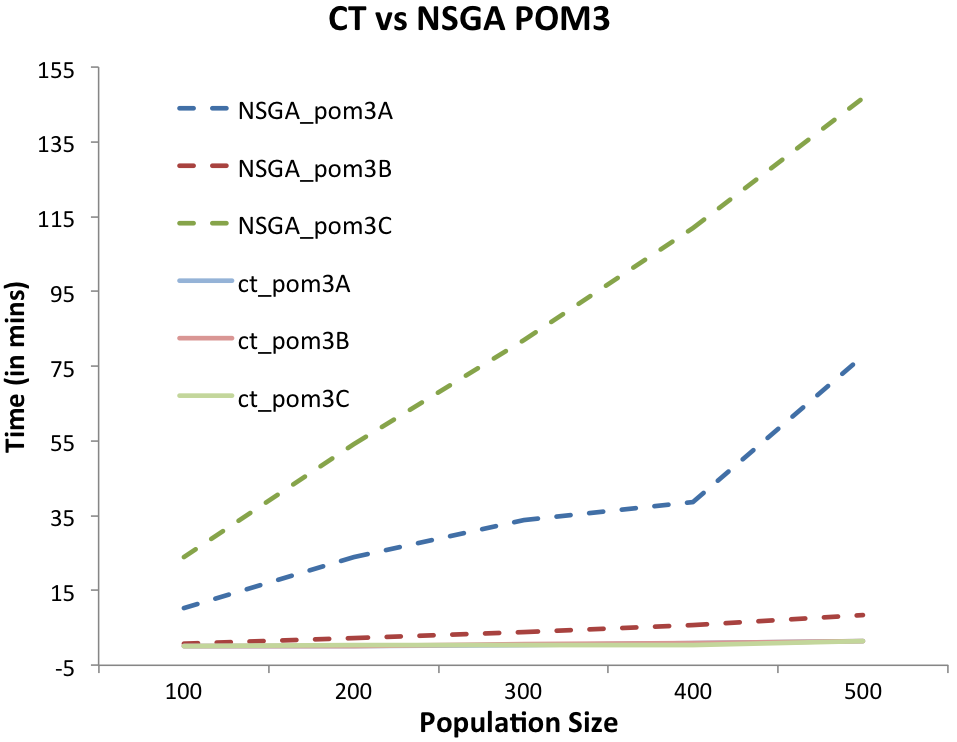
\includegraphics[width=6cm]{naveen/figures/pomtimes.png}
\caption{ Runtimes (minutes) for CT and NSGA II on POM Model
(means over 20 repeats)}\label{fig:pomtimes}
\end{figure}

Note that these runtime results come from an optimized version of WICKED.
Experiments are on-going with the Python profiler 
(to remove runtime bottlenecks). While those initial results are promising, we have
nothing definitive to report at this time.

\subsection{Optimization Improvements}

To explore optimization improvements, we:
\be
\item
Collected
{\em baseline}  distributions seen in the objectives of the initial population
(of 25 randomly generated individuals). 
\item Using the baseline as generation $G=1$, run NSGA-II until
no improvement in any objective for three generations;
\item Using that baseline, run WICKED once. For each cluster:
\bi
\item
Access the cluster items and the recommendation from the cluster;
\item
Re-run the model that generated the data using constraints
generated from that cluster; 
 \ei
\item Collected {\em treated} distributions from the output
of steps two and three.
\ee

\fig{optresults} shows the {\em baseline} and {\em treated} distributions
for:
\bi
\item For all the objectives of:
\bi
\item The three variants of POM3 shown in \fig{POM3abcd};
\item The three variants of XOMO shown in \fig{xomocases};
\ei
\ei
That figure presents displays results from 20
repeated runs as horizontal quartile charts. In that
figure, black dots denote median values and
horizontal lines denote the 25 to 75th percentile
range.  To simplify readability, for each objective,
all results and normalized 0..100 for the min to max
values seen for that objective.  Our three
treatments are shown in the ``Rx'' column: ``0''
denotes the baseline; ``W'' denotes WICKED, and
``N'' denotes NSGA-II.

In all these results, {\em lower} values are {\em
better} (exception: the {\em completion} goal in
POM3 which we seek to {\em maximize}). 

\renewcommand{\baselinestretch}{0.4}
\begin{figure}[!t]
\scriptsize
%\bf
\begin{minipage}{.52\linewidth}


\begin{tabular}{|l@{~}c@{~}c@{~}r|}
\arrayrulecolor{lightgray}
\rowcolor[gray]{.85} Fl     & Rx  & median &  \\ 
\rowcolor[gray]{1.0} effort  & 0 & 19 &  \quart{8.0}{15.0}{19.0} \\ 
 & W & 4 & \quart{0.0}{5.0}{4.0} \\ 
 & N & 11 &  \quart{4.0}{12.0}{11.0} \\ 
\hline\rowcolor[gray]{1.0} months  & 0 & 27 &  \quart{20.0}{1.0}{27.0} \\ 
 & W & 19 & \quart{15.0}{0.0}{19.0} \\ 
 & N & 36 &  \quart{27.0}{13.0}{36.0} \\ 
\hline\rowcolor[gray]{1.0} defects  & 0 & 22 &  \quart{10.0}{29.0}{22.0} \\ 
 & W & 2 & \quart{0.0}{3.0}{2.0} \\ 
 & N & 5 &  \quart{1.0}{7.0}{5.0} \\ 
\hline\rowcolor[gray]{1.0} risks  & 0 & 87 &  \quart{82.0}{5.0}{87.0} \\ 
 & W & 2 &  \quart{0.0}{0.0}{2.0} \\ 
 & N & 6 &  \quart{1.0}{9.0}{6.0} \\ 
\end{tabular}



\begin{tabular}{|l@{~}c@{~}c@{~}r|}
\arrayrulecolor{lightgray}
\rowcolor[gray]{.85}  GR  &Rx & median  &  \\ 
\rowcolor[gray]{1.0} effort  
 & 0 & 7 & \quart{3.0}{5.0}{7.0} \\ 
 & W & 3 &  \quart{0.0}{3.0}{3.0} \\ 
 & N & 13 &  \quart{6.0}{14.0}{13.0} \\ 
\hline\rowcolor[gray]{1.0} months  
 & 0 & 21 & \quart{17.0}{0.0}{21.0} \\ 
 & W & 23 &  \quart{18.0}{2.0}{23.0} \\ 
 & N & 39 &  \quart{29.0}{16.0}{39.0} \\ 
\hline\rowcolor[gray]{1.0} defects  
 & 0 & 16 &  \quart{7.0}{22.0}{16.0} \\ 
 & W & 1 &  \quart{0.0}{2.0}{1.0} \\ 
 & N & 4 &  \quart{1.0}{5.0}{4.0} \\ 
\hline\rowcolor[gray]{1.0} risks  
 & 0 & 74 &  \quart{66.0}{13.0}{74.0} \\ 
 & W & 6 &  \quart{3.0}{3.0}{6.0} \\ 
 & N & 5 &  \quart{0.0}{8.0}{5.0} \\ 
\end{tabular}



\begin{tabular}{|l@{~}c@{~}c@{~}r|}
\arrayrulecolor{lightgray}
\rowcolor[gray]{.85}02  & Rx & median  &  \\ 
\rowcolor[gray]{1.0} effort  & 0 & 5 &  \quart{3.0}{0.0}{5.0} \\ 
 & W & 7 &  \quart{6.0}{1.0}{7.0} \\ 
 & N & 13 &  \quart{6.0}{14.0}{13.0} \\ 
\hline\rowcolor[gray]{1.0} months  & 0 & 25 &  \quart{23.0}{0.0}{25.0} \\ 
 & W & 20 &  \quart{19.0}{0.0}{20.0} \\ 
 & N & 43 &  \quart{33.0}{20.0}{43.0} \\ 
\hline\rowcolor[gray]{1.0} defects  & 0 & 37 &  \quart{25.0}{24.0}{37.0} \\ 
 & W & 1 &  \quart{1.0}{0.0}{1.0} \\ 
 & N & 5 &  \quart{1.0}{8.0}{5.0} \\ 
\hline\rowcolor[gray]{1.0} risks  & 0 & 79 &  \quart{67.0}{16.0}{79.0} \\ 
 & W & 13 &  \quart{12.0}{0.0}{13.0} \\ 
 & N & 6 &  \quart{0.0}{10.0}{6.0} \\\hline 
\end{tabular}
\end{minipage}\begin{minipage}{.4\linewidth}

\begin{tabular}{|l@{~}c@{~}c@{~}r|}

\arrayrulecolor{lightgray}
\rowcolor[gray]{.85} POM3a  & Rx  & median & \\ 
\rowcolor[gray]{1.0} cost  & 0 & 32  & \quart{19.0}{28.0}{32.0} \\ 
 & W & 35 &  \quart{23.0}{25.0}{35.0} \\ 
 & N & 3 & \quart{3.0}{0.0}{3.0} \\ 
\hline\rowcolor[gray]{1.0} completion  & 0 & 85 &  \quart{74.0}{2.0}{85.0} \\ 
 & W & 75 &  \quart{65.0}{0.0}{75.0} \\ 
 & N & 86 &  \quart{78.0}{1.0}{86.0} \\ 
\hline\rowcolor[gray]{1.0} idle  & 0 & 22 & \quart{1.0}{36.0}{22.0} \\ 
 & W & 17 &  \quart{0.0}{29.0}{17.0} \\ 
 & N & 31 &  \quart{4.0}{45.0}{31.0} \\ 
\end{tabular}


\begin{tabular}{|l@{~}c@{~}c@{~}r|}
\arrayrulecolor{lightgray}
\rowcolor[gray]{.85} POM3B  & Rx & median &  \\ 
\rowcolor[gray]{1.0} cost  & 0 & 32 &  \quart{20.0}{27.0}{32.0} \\ 
 & W & 19 &  \quart{12.0}{14.0}{19.0} \\ 
 & N & 6 &  \quart{5.0}{0.0}{6.0} \\ 
\hline\rowcolor[gray]{1.0} completion  & 0 & 84 &  \quart{74.0}{2.0}{84.0} \\ 
 & W & 55 &  \quart{47.0}{0.0}{55.0} \\ 
 & N & 86 &  \quart{77.0}{2.0}{86.0} \\ 
\hline\rowcolor[gray]{1.0} idle  & 0 & 29 &  \quart{5.0}{37.0}{29.0} \\ 
 & W & 17 &  \quart{0.0}{27.0}{17.0} \\ 
 & N & 32 &  \quart{6.0}{47.0}{32.0} \\ 
\end{tabular}





\begin{tabular}{|l@{~}c@{~}c@{~}r|}
\arrayrulecolor{lightgray}
\rowcolor[gray]{.85} POM3C    & Rx & median & \\ 
\rowcolor[gray]{1.0} cost  & 0 & 40 &  \quart{27.0}{25.0}{40.0} \\ 
 & W & 31 &  \quart{20.0}{20.0}{31.0} \\ 
 & N & 10 &  \quart{8.0}{0.0}{10.0} \\ 
\hline\rowcolor[gray]{1.0} completion  & 0 & 90 &  \quart{82.0}{0.0}{90.0} \\ 
 & W & 63 & \quart{54.0}{1.0}{63.0} \\ 
 & N & 90 &  \quart{83.0}{1.0}{90.0} \\ 
\hline\rowcolor[gray]{1.0} idle  & 0 & 34 &  \quart{8.0}{33.0}{34.0} \\ 
 & W & 21 &  \quart{0.0}{25.0}{21.0} \\ 
 & N & 36 &  \quart{8.0}{41.0}{36.0} \\\hline
\end{tabular}~\\\vspace{2.11cm}~\\\end{minipage}

\caption{  XOMO results (left); POM3 results (right);
all results from 20 runs with different random seeds.
Big black dots show median values. 
Horizontal
lines show 25th to 75th percentile.
All results are normalized 0..100, min..max. 
Except for POM3's {\em completion} objective, 
{\em smaller} values are
{\em better}. In the ``Rx'' column,
``0,W,N'' denotes 
results from baseline,
WICKED, and  NSGA-II (respectively).
}\label{optresults}
\end{figure}
\renewcommand{\baselinestretch}{1}

